\RequirePackage{luatex85}
\PassOptionsToPackage{shorthands=off}{babel}
\makeatletter
\disable@package@load{fontenc}
\makeatother
\let\oldlooseness=\looseness
\documentclass{csbulletin}
\selectlanguage{czech}
\setcounter{secnumdepth}{3}
\usepackage{titlesec}
\titlelabel{\thetitle\enspace}
\usepackage{luavlna}
\usepackage[strict]{lua-widow-control}
\usepackage{graphicx}
\graphicspath{{}{img/}}
\usepackage{ragged2e}
\usepackage{fontspec}
\setmainfont{Latin Modern Roman}[
  SmallCapsFont = Latin Modern Roman Caps,
  BoldFeatures = {SmallCapsFont = {CMU Serif Bold}},
  ItalicFeatures = {SmallCapsFont = {CMU Serif Roman Slanted}},
  BoldItalicFeatures = {SmallCapsFont = {CMU Serif Bold Slanted}},
  SmallCapsFeatures = {Letters = SmallCaps},
]
\usepackage{fontawesome5}
\directlua{luaotfload.add_fallback
("emojifallback",
  {"NotoColorEmoji:mode=harf"}
)}
\setmonofont{Latin Modern Mono}[RawFeature={fallback=emojifallback}]
\usepackage{tabularx,booktabs}
\usepackage{xcolor,minted}
% \usemintedstyle{bw}
\AtBeginEnvironment{minted}{\let\textit\textsl\let\itshape\slshape}
\AtBeginEnvironment{tcolorbox}{\let\textit\textsl\let\itshape\slshape}
%These are the background colors of the boxes
\colorlet{CommentColBack}{black!2}
\colorlet{ListingColBack}{black!8}
\colorlet{TextColBack}{black!4}
\colorlet{TitleColBack}{white}

\makeatletter
\renewenvironment{minted@snugshade*}[1]{%
  \def\FrameCommand##1{\hskip\@totalleftmargin
    \colorbox{#1}{##1}\llap{\raisebox{.5ex}[0pt][0pt]{\listingIcon\hspace*{1ex}}}
    %
    \hskip-\linewidth \hskip-\@totalleftmargin \hskip\columnwidth}%
  \MakeFramed{\advance\hsize-\width
    \@totalleftmargin\z@ \linewidth\hsize
    \advance\labelsep\fboxsep
    \@setminipage}%
 }{\par\unskip\@minipagefalse\endMakeFramed}

\makeatother
\newcommand*{\setListingIcon}[1]{\def\listingIcon{#1}}
\setListingIcon{}
\AtBeginDocument{
  \newlength{\mintednumbersep}
  \sbox0{\tiny00}%
  \setlength\mintednumbersep{1em}%
  \addtolength\mintednumbersep{-\wd0}%
  \setminted{numbersep=\mintednumbersep}
}
\setminted{xleftmargin=1em,numbers=left,breakaftersymbolpre={},bgcolor=ListingColBack}
\usepackage{csquotes}
\usepackage[
  backend=biber,
  style=iso-numeric,
  sortlocale=cs,
  autolang=other,
  bibencoding=UTF8,
  mincitenames=2,
  maxcitenames=2,
  doi=true,
  isbn=false,
  shortnumeration=true,
]{biblatex}
\renewcommand\multicitedelim{\addsemicolon\space}
\addbibresource{peischl-pipeline.bib}
\usepackage[implicit=false,hidelinks]{hyperref}

% Document commands [MP et al.]
\DeclareRobustCommand\meta[1]{%
  \ensuremath{\langle}%
  \ifmmode \expandafter\mbox \fi % if in math
  {\it #1\/}% no typewriter italics, please
  \ensuremath{\rangle}%
}
\def\faForgejo{%
  
\includegraphics[height=1\ht\strutbox, alt={Černobílá verze ikony Forgejo}]{forgejo-icon}%
}
\NewDocumentCommand{\GitHub}{s}{%
  \faIcon{github}%
}
\NewDocumentCommand{\GitLab}{s}{%
  \faIcon{gitlab}%
}
\NewDocumentCommand{\Forgejo}{s}{%
  \faIcon{forgejo}%
}

% Document commands [VSN]
\ExplSyntaxOn
\DeclareRobustCommand
  \acro
  [ 1 ]
  {
    \tl_set:Nn
      \l_tmpa_tl
      { #1 }
    \regex_replace_all:nnN
      { [^\d]+ }
      { \c{textsc} \cB\{ \c{MakeLowercase} \cB\{ \0 \cE\} \cE\} }
      \l_tmpa_tl
    \regex_replace_all:nnN
      { \d+ }
      { \c{oldstylenums} \cB\{ \0 \cE\} }
      \l_tmpa_tl
    \tl_use:N
      \l_tmpa_tl
  }
\ExplSyntaxOff
\makeatletter
\DeclareRobustCommand{\La}{L\kern-.36em%
        {\sbox\z@ T%
         \vbox to\ht\z@{\hbox{\check@mathfonts
                              \fontsize\sf@size\z@
                              \math@fontsfalse\selectfont
                              A}%
                        \vss}%
        }}
\makeatother
\def\AllTeX{(\La\kern-.075em)\kern-.075em\TeX}
\babelhyphenation[czech]{Git-Hub Git-Hubu}

\begin{document}

\singlechars{czech}{AaIiVvOoUuSsZzKk}

\title{Příprava \AllTeX ových dokumentů v cloudu}
\EnglishTitle{Creation of \LaTeX{} documents using a cloud-based pipeline}
\author{Marei Peischl, Marcel Krüger a Oliver Kopp}
\podpis{\begin{minipage}[t]{3.5cm}\raggedleft
Marei Peischl \\ Gneisenaustr. 18 \\ 202~53 Hamburk \\ Německo \\ \url{marei@peitex.de} \\ \url{https://peitex.de}
\end{minipage}\begin{minipage}[t]{2.85cm}\raggedleft
Marcel Krüger \\ Hamburk \\ Německo
\end{minipage}\kern-5em\relax\begin{minipage}[t]{4.25cm}\raggedleft
Oliver Kopp \\ Sindelfingen \\ Německo
\end{minipage}}

\maketitle[1ex]

\begin{abstract}
Používání webových služeb pro kolaborativní přípravu dokumentů v \AllTeX u je dnes běžné, ale tyto nástroje se zaměřují na psaní dokumentů, nikoliv na tvorbu šablon nebo balíčků. Používání serverů pro průběžnou integraci a doručení je běžné ve vývoji softwaru, ale může být snadno přizpůsobeno pro \TeX{} a přátele.

Tento článek ukazuje, jak začít s používáním automatizace na webových službách jako GitHub, Forgejo nebo GitLab, a to jak pro autory dokumentů, tak pro vývojáře \AllTeX ových balíčků.
\end{abstract}
\klicovaslova: průběžná integrace a doručení, GitHub, Forgejo, GitLab, docker

\makeatletter
\def\@thefnmark{}\@footnotetext{Z~anglického originálu \cite{peischl2024pipeline} přeložil a rozšířil se svolením autorů a vydavatele Vít S. Novotný.}
\makeatother

\vspace{-2pt}
\section{Úvod}
\vspace{-1pt}
Všechno se dnes přesouvá do cloudu nebo je tam již dostupné.
\AllTeX{} je v cloudu již přibližně 10 let a dnes je zcela běžné používat pro přípravu dokumentů webový editor (jako Overleaf~\cite{novotny2021overleaf,stano2024overleaf}, pozn. red.), zatímco kompilace na vlastním počítači se stala \enquote{záležitostí geeků}.
Existuje však také třetí varianta pro kompilaci \AllTeX ových dokumentů, kterou můžeme využít také ke zlepšení procesu vývoje balíčků a obecně ke zvýšení stability \AllTeX u: osvojení metod DevOps, jako je průběžná integrace a doručení (tzv. \acro{CI/CD}) s použitím automatizovaných postupů.

Pracovně můžeme definovat postup \acro{CI/CD} (anglicky ,,workflow``, pozn. překl.) jako soubor kroků, které vedou ke kompilaci \AllTeX ového dokumentu do formátu \acro{PDF} na nějaké online službě, která má přístup ke zdrojovým souborům.

\vspace{-2pt}
\section{Proč průběžná integrace?}
\vspace{-1pt}
Zaběhnuté pracovní postupy nás často odrazují od změn v našem způsobu práce. Aby tedy mělo smysl číst tento článek, natož pak integrovat tyto mechanismy do projektů, musí pro to existovat dobré důvody.

Raní uživatelé postupů \acro{CI/CD} v ekosystému \TeX u se snažili držet krok se současným stavem ve světě open source softwaru a otevřít dveře přispěvatelům do vývojového procesu. Například projekt \LaTeX{} interaguje s uživateli prostřednictvím projektů na webové službě GitHub~\cite{latex3-github}. Přijímá zde také příspěvky v podobě softwarových záplat, ze kterých může těžit celá \AllTeX ová komunita.

Výhody těchto metod však sahají mnohem dál. Zaměříme se na několik vybraných aspektů, protože vyčerpávající popis by vydal na samostatný článek.

\vspace{-1pt}
\subsection{U mě to funguje?!}
Někdy se mi na mém počítači podaří úspěšně zkompilovat dokument, ale mému vedoucímu na jeho počítači už ne. Existuje mnoho důvodů, proč může kompilace \TeX ového dokumentu na jednom systému uspět a na jiném selhat. Spuštění externího průběžného integračního procesu nejenže ilustruje veškeré potřebné kroky pro přechod od zdrojových souborů k výstupu ve formátu \acro{PDF}, ale také pomůže zjistit, zda jsou problémy specifické pro konkrétní počítač, nebo zda jsou obecné.
\oldlooseness=-1

\vspace{-1pt}
\subsection{Zpětná kompatibilita a regresní testování}
\label{sec:backwards-compatibility}
S použitím postupů \acro{CI/CD} můžeme spustit kompilaci na různých distribucích \TeX u nebo jejich verzích. Díky tomu můžeme otestovat, zda nějaký balíček způsobuje problémy ještě před tím, než např. nainstalujeme nejnovější verzi MiK\TeX u na svém počítači. To nám může ušetřit mnoho času, protože návrat k předchozí verzi je často komplikovaný.\footnote{To je další problém\ldots{} Ale to už je jiný příběh, který by také vystačil na samostatný článek.}

Tuto metodu můžeme také využít ke kontrole zpětné kompatibility, například pokud jeden z přispěvatelů používá stabilní verzi Debianu, která obsahuje pouze zastaralou verzi \TeX ové distribuce. Jak již bylo řečeno, tým projektu \LaTeX{} tyto techniky již mnoho let používá a dokonce poskytuje funkce pro regresní testování v rámci jejich systému l3build~\cite{l3build,l3build-beginner} pro sestavování \AllTeX ových balíčků.

Vývojáři balíčků mohou postupy \acro{CI/CD} používat jako obecné rozhraní pro regresní testování. To pomáhá předcházet některým chybám, které by jinak byly zveřejněny a nalezeny až samotnými uživateli. Dále je možné \acro{CI/CD} postupy použít pro detekci nekonzistencí v kódu. Jeden z autorů např. zjistil, že značné množství balíčků a souborů v distribuci \TeX~Live neuvádí v kódu číslo verze.

\vspace{-3pt}
\section{Struktura článku}
\vspace{-2pt}

Cílem tohoto článku je seznámit čtenáře se základy nastavení postupů \acro{CI/CD} na webových službách GitHub, Forgejo a GitLab. Článek je zaměřen především na dvě skupiny uživatelů:

\begin{enumerate}
\item autory, kteří se zaměřují na sazbu obsahu, a jejich spolupracovníky a
\item vývojáře balíčků a šablon, jejichž práce tvoří podloží pro práci autorů.
\end{enumerate}

Vývojáři samozřejmě mohou využít postupy určené pro autory, například pro sazbu dokumentace balíčku.% Vývojáři tak obvykle používají rozšířenou verzi nastavení určeného pro autory.

Vzhledem k tomu, že všechny služby pokryté tímto článkem jsou založeny na systému správy verzí git, očekáváme, že projekt bude gitový repozitář. Pro čtenáře, kteří dosud git nepoužívají, odkazujeme doplňující informace z repozitáře tohoto článku~\cite{tug2024-cicd-tugboat-sources}. S jejich využitím lze git používat, aniž by si to uživatel vůbec uvědomoval, protože je integrován do automatického ukládání v textovém editoru.

Protože projekt \LaTeX{} používá službu GitHub, začneme podrobným vysvětlením postupů GitHub Actions a poté vytvoříme odpovídající postupy na dalších službách. Všechny postupy \acro{CI/CD} jsou k dispozici v ukázkových repozitářích uvedených v Tabulce~\ref{tab:demo-repos}. Všechny ukázky kódu v tomto článku jsou označeny ikonami, aby nedošlo k záměně, protože služby budeme v článku střídat pro ilustraci rozdílů: Ikona \faGithub{} označuje, že ukázka pochází z postupu GitHub Actions, zatímco ikona \faGitlab{} označuje postup GitLab \acro{CI}.

\begin{table}
\caption{Ukázkové repozitáře zveřejněné spolu s tímto článkem. Názvy repozitářů mají strukturu \meta{typ~postupu}\texttt{\_}\meta{úkol} s přidáním koncovky \texttt{\_minimal} v případě, že příklad nepoužívá předpřipravený dockerový obraz, ale zahrnuje metody instalace balíčků na základě souboru závislostí, jak popisujeme v sekci~\ref{sec:minimize}.
\endgraf\medskip
Všechny zde uvedené varianty jsou připraveny pro alespoň tři zde uvedené webové služby: \,\faGithub{} GitHub, \,\faGitlab{} GitLab a \,\faForgejo{} Forgejo.
\endgraf\medskip
Vzhledem k tomu, že adresy repozitářů jsou poměrně dlouhé, zveřejnili jsme je v repozitáři tohoto článku~\cite{tug2024-cicd-tugboat-sources} na adrese \citefield{tug2024-cicd-tugboat-sources}[citeurl]{url}.}
\label{tab:demo-repos}
\medskip
\input img/demo-repos
\vspace{-6pt}
\end{table}

\vspace{-4pt}
\section{Kompilace dokumentu pomocí průběžné integrace}
\vspace{-2pt}
\subsection{První kroky s GitHub Actions}
\setListingIcon{\GitHub}

Nejprve založíme repozitář na službě GitHub. Repozitář nemusí být veřejný.
Ke kompilaci \AllTeX ového dokumentu v „čistém“ prostředí potřebujeme následující:

\begin{enumerate}
\item Připravit prostředí a nainstalovat \TeX ovou distribuci, např. \TeX~Live.
\item Spustit na dokumentu \TeX ový stroj s příslušným formátem, např. \LaTeX em.
\end{enumerate}

Kromě elementárních příkazů poskytuje služba GitHub předpřipravené ,,akce``, které provádí více elementárních příkazů v jednom kroku. Pro nás je zajímavá např. akce \texttt{latex-action}~\cite{latex-action}, která zkompiluje \LaTeX ový dokument pomocí příkazu \texttt{latexmk} uvnitř kontejneru s instalací \TeX~Live. Tato a další akce však obvykle omezují možnosti konfigurace, aby bylo rozhraní co nejjednodušší.

V článku se budeme zabývat dvěma přístupy: Použitím dockerového obrazu s plnou instalací \TeX~Live v této sekci a s minimální instalací \TeX~Live v Sekci~\ref{sec:minimize}.

Konfigurace postupu \acro{CI/CD} se provádí vytvořením souboru \acro{YAML} v adresáři \texttt{.github/workflows/}. Název souboru můžeme zvolit libovolný, např. \texttt{ahoj-světe.yml}. Následující ukázka kódu zobrazuje minimální konfiguraci:

\inputminted{yaml}{examples/hello-world.yml}

Níže uvádíme význam jednotlivých sekcí souboru \acro{YAML}:

\begin{description}
\item[name:] Název postupu, který bude zobrazený ve webovém rozhraní GitHubu. Tento název je důležitý, pokud projekt obsahuje více postupů.

\item[on:] Podmínky, za kterých bude postup spuštěn.
V naší ukázce se úlohy spustí při každém \texttt{push}i, tj. kdykoliv aktualizujeme obsah repozitáře.
Kromě reakce na změny obsahu je možné spouštět úlohy pravidelně v určitý čas.

Pro všechny možnosti vizte dokumentaci~\cite{github-actions-ref}. Výchozí nastavení se liší pro každou platformu (jako Windows, Linux a Mac~OS, pozn. překl.) a může být specifické pro konkrétní výpočetní uzel, vizte níže.

\item[jobs:] Seznam úloh, které se mají postupně spustit.
Je například běžné mít jednu úlohu pro kompilaci dokumentu a druhou pro zveřenění výsledného souboru \acro{PDF}.
V naší ukázce je jen jedna úloha nazvaná \texttt{ukázková-úloha}.

\item[runs-on:] Nastavení výpočetního uzlu (anglicky ,,runner``, pozn. překl.).
Výpočetní uzly jsou servery, které vykonávají úlohy definované v sekci \texttt{jobs}. Nemusí jít o stejné servery, na kterém jsou hostovány gitové repozitáře.
V naší ukázce označuje \texttt{ubuntu-latest} vestavěný výpočetní uzel poskytovaný službou GitHub, který používá linuxovou distribuci Ubuntu.
Výpočetní uzel obsahuje program NodeJS a některé další nástroje pro usnadnění práce s předdefinovanými akcemi. Úplný seznam vestavěných uzlů najdeme v dokumentaci~\cite{github-hosted-runners}.

\item[steps:] Kroky, tj. elementární příkazy a akce, které má postup skutečně provést. V elementárních příkazech je možné přímo zadávat kód pro příkazovou řádku operačního systému a používat Unicode. Náš elementární příkaz vypíše text na standardní výstup a měl by proběhnout bez problémů.
\end{description}

Na GitHubu jsou postupy pro nové repozitáře automaticky povoleny.
Při použití vestavěného výpočetního uzlu tak, jak to děláme zde, nám pro spuštění postupu stačí do repozitáře přidat soubor \acro{YAML}. Následně se postup spustí při všech následujících změnách obsahu repozitáře.

Aktuální stav postupu, tj. který krok právě běží nebo zda již byl dokončen, lze vždy zkontrolovat na
\meta{adrese repozitáře}\texttt{/actions}. Například stav postupu pro první z našich ukázkových repozitářů najdete na adrese
{\DeclareFieldFormat{citeurlpostfix}{\url{#1/actions}}\citefield{workflow-github}[citeurlpostfix]{url}}. Vypadá nějak takto:
\par
\medskip

\begingroup
\centering
\noindent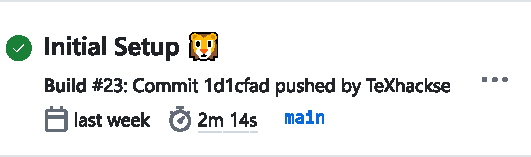
\includegraphics[width=0.7\linewidth,alt={Výřez ze snímku obrazovky stránky stavu postupu CI/CD. Běh byl úspěšný. Commit byl proveden uživatelem @TeXhackse s popisem „Initial setup“ následovaným emotikonem lva.}]{screenshot-pipeline-successful}
\par\medskip
\endgroup

Postup proběhl úspěšně a vypsal text na příkazovou řádku operačního systému. Nyní přejdeme k dalšímu kroku: kompilaci \LaTeX ového dokumentu.

\subsubsection{GitHub Actions s \LaTeX em}

GitHub Actions jsou postaveny na kontejnerizovaném softwaru, který je spouštěný pomocí dockeru. Naštěstí někteří z nás žijí na Ostrově \TeX u (anglicky ,,Island of \TeX``, zkráceně IoT, pozn. překl.) a udržují dockerové obrazy, které zde můžeme využít.\footnote{Velké díky ostatním obyvatelům Ostrova!}
Příprava těchto obrazů byla popsána v~předchozím článku~\cite{islandoftex-docker-short}.

V této sekci upravíme ukázkový postup z předchozí strany tak, aby zkompiloval \LaTeX ový dokument pomocí obrazu od IoT.
První část postupu zůstane prozatím stejná, změny nastávají až po direktivě \texttt{runs-on}:

\inputminted[firstline=5, lastline=12]{yaml}{examples/latex-basic-01.yml}

\begin{description}
\item[container:] Dockerový obraz, uvnitř kterého se spouští veškeré kroky. V našem příkladu jsme zvolili obraz \texttt{texlive/texlive:latest} s plnou instalací \TeX~Live a některými doplňujícími nástroji~\cite{islandoftex-docker}.
\item[steps:] První krok vypadá odlišně od našeho předchozího příkladu. Tento má název „Stáhni repozitář“ a místo elementárního příkazu používá akci \texttt{actions\discretionary{/}{}{/}checkout@v4} z tagu \texttt{v4} gitového repozitáře na adrese~\citefield{github-action-checkout}[citeurl]{url}. Tato akce se stará o autentizaci a některé interní záležitosti, takže se nemusíme těmito detaily zabývat. Veškeré další kroky proběhnou už v kořenovém adresáři staženého repozitáře.\pagebreak

Druhý krok má název ,,Zkompiluj \LaTeX ové dokumenty`` a spouští elementární příkaz stejně jako naše předchozí ukázka. Tentokrát spustíme příkaz \texttt{latexmk}~\cite{latexmk} s volbou \texttt{--lualatex}, která, jak možná tušíte, vynutí použití stroje Lua\TeX{} s formátem \LaTeX.
Ve výchozím nastavení \texttt{latexmk} zpracuje všechny soubory s koncovkou \texttt{.tex} v kořenovém adresáři repozitáře. Díky tomu v direktivě \texttt{run:} nemusíme uvádět jména řídicích souborů našich \LaTeX ových dokumentů. Postačí, když veškeré soubory s koncovkou \texttt{.tex}, které nemají být zkompilovány, umístíme do podadresářů.
\end{description}

\vspace{-13pt}
\subsubsection{Kde jsou soubory \acro{PDF}?}
Pokud byl postup úspěšný, uvidíme sice zelenou ikonu, ale soubory \acro{PDF} bychom hledali marně. Je to proto, že služba GitHub neví, které výstupní soubory chce uživatel skutečně vidět nebo stáhnout. Tyto kýžené soubory se nazývají ,,artefakty``. Nyní přidáme do předchozího postupu další krok s akcí \texttt{actions/upload-artifact@v4}, která soubory \acro{PDF} označí jako artefakty:

\inputminted[firstline=13, lastline=17]{yaml}{examples/latex-basic-01.yml}

Po dalším úspěšném běhu postupu bude možné přistoupit k souborům \acro{PDF}, které budou zabaleny do archivu \acro{ZIP} a dostupné na stránce se stavem běhu. Kliknutím na běh na stránce s přehledem akcí se dostaneme k artefaktu:
\par
\medskip

\begingroup
\centering
\noindent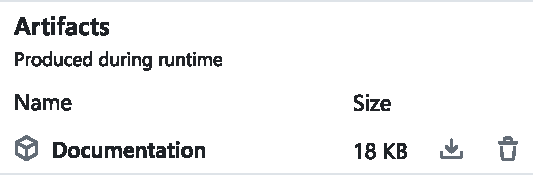
\includegraphics[width=0.6\linewidth,alt={Výřez ze snímku obrazovky, který ukazuje stahování artefaktů na GitHubu. Zde je k dispozici zabalený artefakt nazvaný „Documentation“.}]{screenshot-artifacts}
\par\medskip
\endgroup

Služba GitHub bohužel momentálně nenabízí možnost stáhnout jednotlivé nezabalené soubory a také neumožňuje vytvořit statický odkaz na nejnovější artefakty. (Jiné služby jako GitLab toto umožňují.) K vyřešení tohoto problému a pro snazší přístup k souborům \acro{PDF} na GitHubu je třeba použít další akce. Nejčastější způsob je publikování \acro{PDF} souborů do samostatné gitové větve. Tento mechanismus se obvykle používá k vytváření webových stránek a nazývá se \enquote{github-pages}.
\oldlooseness=-1

Pro zápis do repozitáře je nejprve nutné upravit oprávnění v souboru \acro{YAML}:

\inputminted[firstline=8, lastline=9]{yaml}{examples/latex-basic-02.yml}

Většina akcí, které se používají k nahrávání artefaktů do gitových větví, navíc požaduje adresář namísto jednoho souboru. Proto je nutné všechny soubory přesunout do samostatného adresáře před tím, než tyto akce použijeme:

\inputminted[firstline=15, lastline=23]{yaml}{examples/latex-basic-03.yml}

\noindent
Token na posledním řádku je nutný k tomu, aby postup mohl měnit repozitář.
\oldlooseness=-1

\vspace{-8pt}
\subsection{Rozdíly oproti Forgejo Actions}

Forgejo~\cite{forgejo} je další webová služba pro správu kódu, jejímž cílem je být otevřenější než GitHub. Lze ji provozovat na vlastním serveru a poskytuje mechanismy podobné GitHub Actions. Tyto mechanismy nikdy nebudou fungovat zcela stejně jako na GitHubu, ale jsou až na několik výjimek kompatibilní.

Forgejo nejprve hledá konfigurační soubory v adresáři \texttt{.forgejo/workflows/}. Pokud žádné nenajde, zkouší je hledat v adresáři \texttt{.github/}. Jediný problém, na který pravděpodobně narazíte při použití stejných postupů jako na GitHubu, je ten, že na většině instancí Forgejo buď nejsou dostupné výpočetní uzly, nebo jsou konfigurované odlišně od těch na GitHubu.

Pokud však dokážete nastavit svůj výpočetní uzel na vlastním serveru se stejnými štítky jako na GitHubu, můžete použít stejné konfigurační soubory pro postupy na obou službách~\cite{forgejo-runner-config}. V ukázkových repozitářích na serveru \url{codeberg.org}, což je instance platformy Forgejo, najdete také popis, jak jsou zde konfigurovány výpočetní uzly.

\vspace{-8pt}
\subsection{Kompilace dokumentu pomocí GitLab \acro{CI}}
\setListingIcon{\GitLab}

Postupy GitLab \acro{CI} se příliš neliší od GitHub Actions. Dokonce je zde konfigurace o něco jednodušší, protože některé kroky jako stažení repozitáře se provádí automaticky. Konfigurační soubor musí být umístěn v kořenovém adresáři repozitáře a pojmenován \texttt{.gitlab-ci.yml}. Zde je náš ukázkový postup:

\inputminted{yaml}{examples/latex-basic-gitlab.yml}

Veškeré kroky v postupu GitLab \acro{CI} jsou elementární příkazy, které se vykonají jeden po druhém. Náš ukázkový postup obsahuje jen jeden příkaz pro spuštění příkazu \texttt{latexmk}. Na rozdíl od GitHubu poskytuje GitLab rozhraní, které umožňuje vytvořit statické odkazy na artefakty. Proto soubor \texttt{README.md} v ukázkových repozitářích na GitLabu obsahuje odkaz v následujícím tvaru:

\begin{FlushLeft}
\meta{adresa repozitáře}\nolinkurl{/-/jobs/artifacts/}\meta{gitová větev}\allowbreak\nolinkurl{/browse?job=}\meta{úloha}
\end{FlushLeft}

Takovýto odkaz zobrazí všechny artefakty připojené k dané úloze.
Např. následující odkaz zobrazí všechny artefakty z ukázkového repozitáře na GitLabu~\cite{workflow-document-gitlab}:

\begin{FlushLeft}\advance\rightskip by 0pt plus.3\hsize
{\DeclareFieldFormat{citeurlpostfix}{\nolinkurl{#1/-/jobs/artifacts/main/browse?job=check:+[latest,+lualatex]}}\citefield{workflow-document-gitlab}[citeurlpostfix]{url}}
\end{FlushLeft}

\vspace{-8pt}
\section{Testování s více \TeX ovými distribucemi a s různými stroji}
\vspace{-4pt}
\setListingIcon{\GitHub}

Jak jsme slíbili v Sekci~\ref{sec:backwards-compatibility}, je možné postupy rozšířit pro testování kompilace s různými verzemi \TeX ových distribucí a s různými \TeX ovými stroji.

Další \TeX ové stroje můžeme přidat v samostatných krocích s odlišnými elementárními příkazy. Stejně tak můžeme další stroje použít v samostatných úlohách, nebo dokonce v samostatných konfiguračních souborech. Volba závisí pouze na tom, zda chceme spustit vše zároveň, nebo šetřit prostředky pomocí podmíněného nebo sekvenčního spuštění.

Pro použití různých verzí \TeX~Live poskytuje IoT obrazy \texttt{texlive/texlive} všech historických verzí s tagy \texttt{TL}\meta{verze}\texttt{-historic} a té aktuální s tagem \texttt{latest}:

\inputminted{yaml}{examples/test-on-iot-texlive.yml}

\begin{description}
  \item[matrix:] Seznam uživatelských parametrů a jejich hodnot, který úlohu přemění na šablonu. Při spuštění postupu vygeneruje šablona úlohy pro všechny kombinace hodnot z matice kartézského součinu parametrů. V našem ukázkovém postupu máme jen jeden parametr \texttt{tag} s různými tagy obrazů \texttt{texlive/texlive}. K hodnotě parametru můžeme uvnitř šablony přistupovat pomocí syntaxe \verb|${{ matrix.tag }}|. V našem ukázkovém postupu dojde k vygenerování tří úloh, které budou používat obrazy s \TeX{} Live 2022, 2023 a s poslední dostupnou verzí \TeX{} Live (v době psaní článku \TeX{} Live 2024, pozn. red.). Úplný seznam dostupných obrazů najdeme na adrese~\citefield{islandoftex-docker-gitlab}[citeurl]{url}.
\end{description}

Postupy GitLab \acro{CI} také podporují šablony úloh. Následující ukázkový postup ilustruje spuštění několika \TeX ových strojů na několika různých verzích \TeX{} Live:
\vspace{-14pt}

\setListingIcon{\GitLab}

\begingroup
\let\savetheFancyVerbLine\theFancyVerbLine
\def\codecomment{\hspace*{-3\mintednumbersep}\textnormal{[ \ldots\ přeskočili jsme sekce \texttt{script} a \texttt{artifacts}\ \ldots\ ]}}
\begin{minted}[escapeinside=||,breaklines,breakafter=/]{yaml}
check:
  image: registry.gitlab.com/islandoftex/images/texlive:$TAG
|\gdef\theFancyVerbLine{}\codecomment\gdef\theFancyVerbLine{\addtocounter{FancyVerbLine}{2}}|
  parallel:|\global\let\theFancyVerbLine\savetheFancyVerbLine|
    matrix:
      - TAG: ['TL2022-historic', 'TL2023-historic', 'latest']
        STROJ: ['pdflatex', 'xelatex', 'lualatex']
\end{minted}
\endgroup

\vspace{-4pt}
V tomto případě je syntax pro přístup k hodnotám parametrů podobná syntaxi proměnných příkazové řádky unixových operačních systémů, ale funguje stejně jako syntax v ukázkovém postupu pro GitHub Actions.

\vspace{-12pt}
\section{Použití malého dockerového obrazu}
\vspace{-6pt}
\label{sec:minimize}\setListingIcon{}

V předchozích příkladech jsme pro jednoduchost používali plnou instalaci \TeX~Live.\footnote{Nejde o zcela plnou instalaci: použité obrazy neobsahují dokumentaci ani zdrojové kódy.} Obrazy od IoT dokonce obsahují všechny závislosti doplňujících nástrojů jako arara nebo minted, takže všechny tyto nástroje fungují bez další konfigurace.

Ne vždy ale potřebujeme plnou instalaci \TeX~Live a menší obrazy se stahují rychleji a šetří místo na disku výpočetních uzlů.\footnote{Pokud vás zajímá, jak snížit nikoliv velikost dockerového obrazu, ale dobu kompilace velkého množství dokumentů, pak doporučujeme vaší pozornosti loňský článek od IoT~\cite{islandoftex-docker}.} V takovém případě ale musíme vědět, které balíčky z \TeX~Live potřebujeme nainstalovat pro kompilaci dokumentů\ldots
\oldlooseness=-1

A zde přichází na scénu nástroj \acro{DEPP} pro výpis závislostí v \TeX~Live~\cite{depp} (anglicky ,,DEPendency Printer for \TeX~Live``, pozn. překl.), hrdě vytvořený na Ostrově \TeX u.\footnote{Pokud mluvíte německy, možná vás překvapí, že tento nástroj je chytřejší, než by jeho název napovídal. (,,Depp`` je jihoněmecký výraz pro hlupáka, pozn. překl.)}
Protože se tento článek zaměřuje na postupy \acro{CI/CD}, nebudeme nástroj \acro{DEPP} podrobněji popisovat. Místo toho ukážeme seznam všech balíčků z \TeX~Live potřebný pro kompilaci, který \acro{DEPP} vygeneroval pro náš ukázkový projekt~\cite{tl_packages}:
\oldlooseness=-1
\vspace{-2pt}

\begingroup
% https://github.com/islandoftex/tug2024-workflow-document-github/blob/main/.github/tl_packages#L7
% Note that we added some more packages manually in front:
%  a) latex binaries <-- this is https://gitlab.com/islandoftex/texmf/depp/-/issues/3
%  b) pdftexcmds <-- This is https://gitlab.com/islandoftex/texmf/depp/-/issues/5
%  c) scheme-minimal
\begin{minted}[breaklines,linenos=false,xleftmargin=0pt,escapeinside=||]{text}
# Proudly generated by the Island of TeX's DEPendency Printer|\textnormal{\ldots}|
blindtext |\textnormal{\ldots}|
\end{minted}
\endgroup

\subsection{GitHub Actions}

Na GitHubu je k dispozici několik akcí pro instalaci \TeX~Live jako součást postupu~\cite{marcel-latex-action,teatimeguest-latex-action}.
Díky tomu můžeme použít menší obraz, což zkrátí dobu kompilace:

\setListingIcon{\GitHub}
\begin{minted}[firstnumber=9]{yaml}
      - name: Instaluj TeX Live
          uses: zauguin/install-texlive@v3
          with:
            package_file: .github/tl_packages
\end{minted}

\noindent
Tento úryvek umístíme do sekce \texttt{steps} před kompilaci dokumentů. Direktiva \texttt{package\_file} odkazuje na výstup nástroje \acro{DEPP} nebo na ručně vytvořený seznam balíčků. Direktiva \texttt{container} je nyní nadbytečná a můžeme ji odstranit.

\vspace{-6pt}
\subsection{GitLab \acro{CI}}
\setListingIcon{\GitLab}

Na GitLabu je instalace \TeX~Live trochu složitější, protože nemáme k dispozici akce, ale jen elementární kroky. Repozitář nástroje \acro{DEPP} proto poskytuje skript \texttt{minimal-portable-tl-setup.sh}~\cite{minimal-portable-tl-setup.sh} pro instalaci podle souboru s balíčky:

\begin{minted}[firstnumber=3]{yaml}
  before_script:
    - minimal-portable-tl-setup.sh tl_packages
\end{minted}

\noindent
Tento úryvek umístíme pod direktivu \texttt{image}, kterou můžeme následně změnit na menší dockerový obraz (jako např. \texttt{debian:latest}, pozn. red.).

Další možností je připravit dockerový obraz, který již potřebné balíčky obsahuje. Pokud používáme vlastní výpočetní uzel, obvykle je to nejlepší řešení, protože můžeme obraz udržovat v mezipaměti a aktualizovat ho podle potřeby.

\vspace{-6pt}
\section{Postupy \acro{CI/CD} pro vývojáře balíčků}
\vspace{-6pt}

Jak jsme již zmínili, výhody používání postupů \acro{CI/CD} jsou ještě větší, když je použijeme při vývoji balíčků nebo šablon.
V takovém případě očekáváme, že repozitář bude obsahovat balíček a nějakou konfiguraci pro nástroj \texttt{l3build}.\footnote{Podobné postupy fungují i pro jiné nástroje, ale to již přesahuje rámec tohoto článku.}

\vspace{-6pt}
\subsection{GitHub Actions}
\setListingIcon{\GitHub}
Příkaz \texttt{latexmk} z předchozích ukázek nahradíme příkazem \texttt{l3build}:

\begin{minted}[firstnumber=9,breaklines]{yaml}
      - name: Spusť l3build
        run: l3build check --show-log-on-error -q -H
\end{minted}

\noindent
Tento krok spustí všechny testy balíčku podle konfigurace nástroje \texttt{l3build}.

Protože se jedná o spuštění testovací sady balíčku, artefakty jsou zcela odlišné. Zatímco při kompilaci dokumentu nás zajímá výstup ve formátu \acro{PDF}, v tomto případě je důležitý výstup testů.
Jeden z autorů tohoto článku proto vytvořil akci, která se o tento výstup postará~\cite{marcel-l3build-failure}:

\begin{minted}[firstnumber=11]{yaml}
      - name: Archivuj výstupy neúspěšných testů
        if: ${{ always() }}
        uses: zauguin/l3build-failure-artifacts@v1
        with:
          name: testfiles
          retention-days: 3
\end{minted}

Kromě nahrání artefaktů tento úryvek ilustruje další důležitý bod:
Na rozdíl od \acro{PDF} dokumentu, kde nás zajímá pouze úspěšný výstup, u testovacích sad nás zajímá především výstup z neúspěšných testů.
Přidali jsme proto podmínku \texttt{if: \$\{\{ always() \}\}}. Ta zajistí, že krok bude spuštěn, i když předchozí krok selže.

\subsection{GitLab \acro{CI}}
\setListingIcon{\GitLab}

Jak už jsme zmínili u předchozích ukázek, GitLab nativně podporuje nahrávání artefaktů bez potřeby načítání externích rozšíření:

\begin{minted}[firstnumber=3]{yaml}
  script:
    - l3build check --show-log-on-error -q -H
  artifacts:
    when: on_failure
    paths:
      - ./build/test/*.diff
\end{minted}

Tím se sice zjednodušuje základní nastavení, ale zároveň se snížuje flexibilita.
Pokud bychom například chtěli použít různé artefakty pro úspěšné a neúspěšné kroky, museli bychom pro to použít dvě samostatné úlohy.

\section{Lokální spuštění}
\setListingIcon{}

Během naší prezentace na konferenci \acro{TUG} 2024 jsme si v rychlosti ukázali, jak můžeme postupy \acro{CI/CD} spouštět lokálně. To může být užitečné při ladění, protože máme možnost ručně spouštět jednotlivé kroky, nebo když potřebujeme zajistit, aby lokální prostředí odpovídalo výpočetnímu uzlu.

Pro služby GitHub a Forgejo existuje nástroj \texttt{act}~\cite{act}, který umožňuje spouštět akce z postupů GitHub Actions pomocí dockeru. Služba GitLab pak umožňuje jednoduše nainstalovat výpočetní uzel lokálně. Díky tomu můžeme spouštět postupy GitLab \acro{CI} tak, že v adresáři s repozitářem spustíme příkaz \texttt{gitlab-runner exec}.
\oldlooseness=-1

\section{Toto je průběžný vývoj!}
\vspace{-6pt}

Všechny zde uvedené konfigurace jsou samozřejmě pouze příklady a můžeme je rozšířit podle požadavků projektu. Můžeme spouštět libovolné příkazy, což může být nezbytné zejména u složitějších projektů.

Například při vytváření časopisů je možné průběžně generovat tiskovou a online verzi, výňatky jednotlivých článků i výstupy ve formátu \acro{HTML/EPUB}, přičemž redaktoři musí počkat pouze na kompilaci článku, na kterém právě pracují.

Totéž platí pro studijní materiály, kde můžeme mít vykreslené verze se zahrnutými řešeními i bez nich, nebo dokumenty, které obsahují vzájemně propojené odkazy, a vyžadují proto několik kompilací.

Integrace postupů \acro{CI/CD} s pokročilejší prací s gitem, jako je smysluplný koncept větvení, může také zlepšit spolupráci nebo zjednodušit proces přispívání do open source projektů. To sníží pracovní zátěž správců projektů, protože některé problémy nebude třeba kontrolovat ručně.

\vspace{-12pt}
\section{Závěr, výzva k zapojení a žádost o zpětnou vazbu}
\vspace{-6pt}

V článku jsme si ukázali, jak můžeme používat služby GitHub, Forgejo a GitLab pro kompilaci dokumentů a vývoj balíčků v \AllTeX u. Předvedli jsme si, jak můžeme využít různé verze distribuce \TeX~Live i různé \TeX ové stroje pro usnadnění testování napříč platformami. Také jsme se postarali o to, aby bylo možné přistoupit k výsledným souborům \acro{PDF} nebo k výsledkům testování.

Doufáme, že tato řešení povedou ke zvýšení stability všech částí vývoje v \AllTeX u tím, že usnadní testování balíčků a ušetří čas při kompilaci složitějších projektů.

Pokud spravujete nějaké balíčky, bylo by skvělé, kdybyste mohli zkusit nastavit testy, které by ověřovaly jejich funkčnost proti nejnovějšímu vydání \TeX~Live (v době psaní článku \TeX{} Live 2024, pozn. red.), aktuální vývojové verzi \TeX~Live, nebo dokonce proti testovacím verzím \TeX~Live před dalším vydáním~\cite{pretest}, pro které IoT od roku 2024 připravuje dockerový obraz \texttt{texlive/texlive} s tagem \texttt{pretest}. Pokud narazíte na problémy, rádi vám pomůžeme.

Rádi bychom tento tutoriál dále udržovali a zjednodušili použití automatizace pro uživatele \TeX u a jeho přátel. Pokud objevíte nějaké nejasnosti, budeme rádi, když se nám ozvete, abychom mohli tento tutoriál vylepšit. Tabulka~\ref{tab:demo-repos} na straně \pageref{tab:demo-repos} shrnuje všechny související ukázkové repozitáře.

Vaše příspěvky do tohoto projektu jsou vítány!

\begingroup
\vspace{-12pt}
\section*{\refname}
\vspace{-6pt}
\sloppy
\printbibliography[heading=none]
\endgroup

\let\oldsection\section
\def\section#1{\def\next Summary: ##1\relax{\oldsection{##1}}\next #1\relax}
\begin{summary}
Using web-based platforms for collaborative editing of \LaTeX{} documents is common these days.
These tools focus on writing documents and not on creation of templates or packages.
Using build servers with automated pipelines is common within software development but can easily be adapted for \TeX{} \& friends.

This article will show how to get started using automated workflows on platforms like GitHub, Forgejo, or GitLab for document authors as well as \TeX{} developers.
\keywords: continuous integration \& delivery, GitHub, Forgejo, GitLab, docker
\end{summary}
\end{document}
